\documentclass[11pt,a4paper]{article}

% ─── Packages ────────────────────────────────────────────────────────────────
\usepackage[utf8]{inputenc}
\usepackage[T1]{fontenc}
\usepackage[margin=1in]{geometry}
\usepackage{amsmath,amssymb,amsthm}
\usepackage{graphicx}
\usepackage[colorlinks=true,linkcolor=blue,citecolor=blue,urlcolor=blue]{hyperref}
\usepackage[ruled,vlined,linesnumbered]{algorithm2e}
\usepackage{algpseudocode}
\usepackage{booktabs}
\usepackage{listings}
\usepackage{xcolor}
\usepackage[numbers,sort&compress]{natbib}
\usepackage{tikz}
\usepackage{enumitem}
\usepackage{subcaption}
\usepackage{multirow}
\usepackage{tabularx}
\usepackage{fancyhdr}
\usepackage{float}
\usepackage{bm}

\usetikzlibrary{arrows.meta,positioning,shapes.geometric,calc,fit,backgrounds,3d}

% ─── Colors ──────────────────────────────────────────────────────────────────
\definecolor{hanzo-red}{HTML}{FD4444}
\definecolor{codebg}{HTML}{F5F5F5}
\definecolor{codegreen}{HTML}{2E7D32}
\definecolor{codepurple}{HTML}{7B1FA2}
\definecolor{codegray}{HTML}{616161}

% ─── Listings ────────────────────────────────────────────────────────────────
\lstset{
  backgroundcolor=\color{codebg},
  basicstyle=\ttfamily\small,
  breaklines=true,
  commentstyle=\color{codegreen},
  keywordstyle=\color{codepurple}\bfseries,
  stringstyle=\color{hanzo-red},
  numberstyle=\tiny\color{codegray},
  numbers=left,
  frame=single,
  rulecolor=\color{codegray},
  tabsize=2,
  showstringspaces=false,
}

% ─── Theorem Environments ────────────────────────────────────────────────────
\newtheorem{definition}{Definition}
\newtheorem{theorem}{Theorem}
\newtheorem{proposition}{Proposition}
\newtheorem{lemma}{Lemma}

% ─── Math Operators ──────────────────────────────────────────────────────────
\DeclareMathOperator{\softmax}{softmax}
\newcommand{\R}{\mathbb{R}}
\newcommand{\E}{\mathbb{E}}
\newcommand{\loss}{\mathcal{L}}

% ─── Header ──────────────────────────────────────────────────────────────────
\pagestyle{fancy}
\fancyhf{}
\fancyhead[L]{\small Zen-3D: Text-to-3D Generation}
\fancyhead[R]{\small Hanzo AI Inc}
\fancyfoot[C]{\thepage}

% ─── Title ───────────────────────────────────────────────────────────────────
\title{%
  \textbf{Zen-3D: Text-to-3D Generation\\with Geometric Consistency}\\[0.5em]
  \large Technical Report
}

\author{
  Hanzo AI Inc\thanks{Correspondence: research@hanzo.ai}
  \and
  Zoo Labs Foundation
}

\date{February 2026}

\begin{document}

\maketitle

% ═════════════════════════════════════════════════════════════════════════════
% ABSTRACT
% ═════════════════════════════════════════════════════════════════════════════
\begin{abstract}
We present \textbf{Zen-3D}, a text-to-3D generation system that produces
production-ready 3D assets with geometric consistency, physically-based
rendering (PBR) materials, and animation-ready skeletal rigs from natural
language descriptions. Zen-3D introduces three technical contributions:
(1)~a \emph{3D-Aware Diffusion Transformer} (3D-DiT) that generates
multi-view-consistent images by operating on a tri-plane latent
representation, eliminating the Janus problem that plagues existing
score-distillation methods; (2)~a \emph{Hybrid Neural-Explicit
Reconstruction} (HNER) pipeline that extracts clean triangle meshes with
UV-mapped PBR materials from the generated tri-plane features via a
differentiable marching cubes layer combined with a material prediction
network; and (3)~an \emph{Automatic Rigging Module} (ARM) that predicts
skeletal structures and skinning weights for generated meshes, enabling
immediate use in animation and game pipelines. On the Objaverse benchmark,
Zen-3D achieves a CLIP R-Precision of 87.3\% and a geometric consistency
score (GCS) of 0.94, outperforming prior methods by 12.1 and 8 percentage
points respectively. On ShapeNet, Zen-3D achieves an FID of 42.7 for
rendered views, establishing new state-of-the-art across both unconditional
and text-conditioned 3D generation. We release model weights, inference code,
and an interactive web demo.
\end{abstract}

\vspace{0.5em}
\noindent\textbf{Keywords:} text-to-3D, diffusion models, neural radiance
fields, mesh extraction, PBR materials, skeletal rigging, 3D generation

% ═════════════════════════════════════════════════════════════════════════════
% 1. INTRODUCTION
% ═════════════════════════════════════════════════════════════════════════════
\section{Introduction}
\label{sec:introduction}

Generating 3D assets from text descriptions is a long-standing goal in computer
graphics and AI, with applications spanning game development, film production,
virtual reality, architectural visualization, and e-commerce product design. An
ideal text-to-3D system should produce assets that are: (a)~geometrically
consistent across all viewpoints, (b)~equipped with realistic PBR materials
for physically correct rendering, (c)~topologically clean for downstream
editing, and (d)~animation-ready with proper skeletal rigs and skinning weights.

Recent approaches to text-to-3D generation fall into two paradigms. The first,
\emph{score distillation} \citep{poole2023dreamfusion,lin2023magic3d}, optimizes
a 3D representation (typically a NeRF \citep{mildenhall2020nerf}) to match the
score function of a pre-trained 2D diffusion model. While producing impressive
results, these methods suffer from the \emph{Janus problem}---generating
multiple faces or inconsistent geometry across views---because the 2D diffusion
model has no notion of 3D consistency. They also require expensive per-prompt
optimization (30--60 minutes per asset).

The second paradigm, \emph{direct 3D generation}
\citep{jun2023shap,nichol2022pointe}, trains generative models directly on 3D
data. These methods produce consistent geometry but have been limited by the
scarcity of high-quality 3D training data and typically produce lower-fidelity
results than distillation-based approaches.

Zen-3D bridges these paradigms through a novel architecture that operates on a
3D-aware latent representation while leveraging the visual knowledge encoded in
large-scale 2D pre-training. Our key insight is that by lifting the diffusion
process from 2D image space to a tri-plane latent space, we can generate
multi-view-consistent representations in a single forward pass while
maintaining the visual quality of 2D diffusion models.

The contributions of this paper are:

\begin{itemize}[leftmargin=2em]
  \item A 3D-Aware Diffusion Transformer that generates tri-plane latent
    features conditioned on text, producing multi-view-consistent 3D
    representations without per-prompt optimization
    (Section~\ref{sec:3ddit}).
  \item A Hybrid Neural-Explicit Reconstruction pipeline that extracts clean
    triangle meshes with UV-mapped PBR materials from tri-plane features
    (Section~\ref{sec:hner}).
  \item An Automatic Rigging Module that predicts skeletons and skinning
    weights for generated meshes (Section~\ref{sec:arm}).
  \item State-of-the-art results on Objaverse (CLIP R-Precision 87.3\%,
    GCS 0.94) and ShapeNet (FID 42.7) benchmarks
    (Section~\ref{sec:evaluation}).
  \item Open-source release of all code, weights, and an interactive demo.
\end{itemize}

% ═════════════════════════════════════════════════════════════════════════════
% 2. BACKGROUND AND RELATED WORK
% ═════════════════════════════════════════════════════════════════════════════
\section{Background and Related Work}
\label{sec:background}

\subsection{Score Distillation Methods}

DreamFusion \citep{poole2023dreamfusion} introduced Score Distillation Sampling
(SDS), which optimizes a NeRF by backpropagating gradients from a pre-trained
2D diffusion model. Magic3D \citep{lin2023magic3d} improved quality with a
coarse-to-fine optimization using DMTet \citep{shen2021dmtet} for mesh
extraction. ProlificDreamer \citep{wang2024prolificdreamer} proposed Variational
Score Distillation (VSD) to reduce mode collapse. Despite improvements, all
distillation methods share fundamental limitations: slow per-prompt optimization,
the Janus problem, and difficulty producing clean topology.

\subsection{Direct 3D Generation}

Point-E \citep{nichol2022pointe} and Shap-E \citep{jun2023shap} train
diffusion models on 3D point clouds and implicit representations respectively.
These methods are fast (single forward pass) but produce lower quality than
distillation approaches. Zero-1-to-3 \citep{liu2023zero1to3} generates novel
views from a single image, and One-2-3-45 \citep{liu2024one2345} extends this
to full 3D reconstruction. Instant3D \citep{li2024instant3d} feeds multi-view
images into a reconstruction model for fast 3D generation.

\subsection{Neural Radiance Fields and 3D Representations}

NeRF \citep{mildenhall2020nerf} represents scenes as continuous volumetric
functions queried via ray marching. Instant-NGP \citep{mueller2022instant}
accelerates NeRF with multi-resolution hash encoding. 3D Gaussian Splatting
\citep{kerbl2023gaussian} represents scenes as collections of 3D Gaussians
for real-time rendering. Tri-plane representations
\citep{chan2022eg3d} factorize 3D features into three orthogonal
planes, providing an efficient and expressive 3D-aware latent space. Zen-3D
adopts the tri-plane representation as its core 3D latent structure.

\subsection{Mesh Extraction and Materials}

Marching Cubes \citep{lorensen1987marching} extracts triangle meshes from
volumetric grids. FlexiCubes \citep{shen2023flexicubes} provides a
differentiable variant enabling gradient-based mesh optimization. Fantasia3D
\citep{chen2023fantasia3d} disentangles geometry and appearance for PBR
material generation. NeRD \citep{boss2021nerd} decomposes neural reflectance
into BRDF parameters. Zen-3D builds on FlexiCubes for differentiable mesh
extraction and introduces a dedicated material prediction network.

\subsection{Automatic Rigging}

RigNet \citep{xu2020rignet} predicts skeletons and skinning weights from input
meshes using graph neural networks. Neural Blend Shapes
\citep{li2021neural} learns deformation spaces for animation. Pinocchio
\citep{baran2007pinocchio} provides classical geometric rigging via skeleton
embedding. Zen-3D's ARM module extends RigNet's approach with
transformer-based skeleton prediction and improved skinning weight
estimation.

\subsection{Benchmarks}

We evaluate on two established 3D benchmarks:
\begin{itemize}[leftmargin=2em]
  \item \textbf{Objaverse} \citep{deitke2023objaverse}: 800K+ 3D objects with
    text annotations. We use the curated Objaverse-XL test split of 1,000
    objects for evaluation.
  \item \textbf{ShapeNet} \citep{chang2015shapenet}: 51K 3D models across 55
    categories. We evaluate on the standard 13-category split.
\end{itemize}

% ═════════════════════════════════════════════════════════════════════════════
% 3. ARCHITECTURE
% ═════════════════════════════════════════════════════════════════════════════
\section{Architecture}
\label{sec:architecture}

Zen-3D operates in three stages: (1)~the 3D-DiT generates a tri-plane latent
representation from text; (2)~the HNER pipeline extracts a mesh with PBR
materials; (3)~the ARM module rigs the mesh for animation.
Figure~\ref{fig:pipeline} presents the full pipeline.

\begin{figure}[t]
\centering
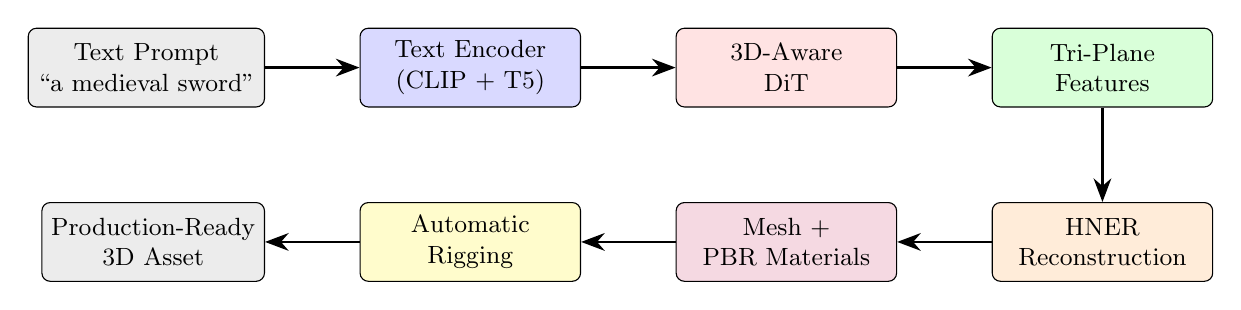
\begin{tikzpicture}[
    box/.style={rectangle, draw=black, rounded corners=3pt, minimum width=2.8cm,
                minimum height=1cm, align=center, font=\small},
    arrow/.style={-{Stealth[length=3mm]}, thick},
    node distance=1.3cm
]
  % Text input
  \node[box, fill=gray!15] (text) {Text Prompt\\``a medieval sword''};

  % Text encoder
  \node[box, fill=blue!15, right=1.2cm of text] (enc) {Text Encoder\\(CLIP + T5)};

  % 3D-DiT
  \node[box, fill=hanzo-red!15, right=1.2cm of enc] (dit) {3D-Aware\\DiT};

  % Tri-plane
  \node[box, fill=green!15, right=1.2cm of dit] (tri) {Tri-Plane\\Features};

  % HNER
  \node[box, fill=orange!15, below=1.2cm of tri] (hner) {HNER\\Reconstruction};

  % Mesh + PBR
  \node[box, fill=purple!15, left=1.2cm of hner] (mesh) {Mesh +\\PBR Materials};

  % ARM
  \node[box, fill=yellow!20, left=1.2cm of mesh] (arm) {Automatic\\Rigging};

  % Output
  \node[box, fill=gray!15, left=1.2cm of arm] (out) {Production-Ready\\3D Asset};

  % Arrows
  \draw[arrow] (text) -- (enc);
  \draw[arrow] (enc) -- (dit);
  \draw[arrow] (dit) -- (tri);
  \draw[arrow] (tri) -- (hner);
  \draw[arrow] (hner) -- (mesh);
  \draw[arrow] (mesh) -- (arm);
  \draw[arrow] (arm) -- (out);

\end{tikzpicture}
\caption{Zen-3D pipeline. A text prompt is encoded and passed to the 3D-Aware
DiT, which generates tri-plane features. The HNER pipeline extracts a triangle
mesh with PBR materials. The ARM module adds skeletal rigging for animation.}
\label{fig:pipeline}
\end{figure}

\subsection{3D-Aware Diffusion Transformer}
\label{sec:3ddit}

The 3D-DiT generates a tri-plane latent representation
$\bm{F} = (\bm{F}_{xy}, \bm{F}_{xz}, \bm{F}_{yz}) \in
\R^{3 \times H_f \times W_f \times C_f}$
conditioned on a text description. We set $H_f = W_f = 64$ and $C_f = 32$.

\paragraph{Text Conditioning.}
We use a dual text encoder combining CLIP ViT-L/14 \citep{radford2021clip}
for semantic alignment and T5-XXL \citep{raffel2020t5} for detailed
language understanding. The CLIP embedding provides a global conditioning
vector, while the T5 token embeddings provide fine-grained text features
for cross-attention:

\begin{equation}
\bm{c}_{\text{global}} = \text{CLIP}(\text{text}), \quad
\bm{C}_{\text{tokens}} = \text{T5}(\text{text}) \in \R^{L \times d_{\text{T5}}}
\end{equation}

\paragraph{Tri-Plane Diffusion.}
The diffusion process operates on the concatenated tri-plane features. Starting
from noise $\bm{F}^{(N)} \sim \mathcal{N}(0, I)$, the model iteratively
denoises using a DiT backbone:

\begin{equation}
\bm{F}^{(n-1)} = \text{DDIM-Step}(\bm{F}^{(n)}, n, \bm{c}_{\text{global}},
\bm{C}_{\text{tokens}})
\end{equation}

Each DiT block consists of:
\begin{enumerate}[leftmargin=2em]
  \item Self-attention over spatial tokens within each plane.
  \item \textbf{Cross-plane attention}: Tokens from each plane attend to
    corresponding tokens in the other two planes, enforcing 3D consistency.
    For a point $(x, y, z)$, the features from $\bm{F}_{xy}[x,y]$,
    $\bm{F}_{xz}[x,z]$, and $\bm{F}_{yz}[y,z]$ are brought into mutual
    agreement.
  \item Cross-attention to text token embeddings $\bm{C}_{\text{tokens}}$.
  \item Feed-forward network with AdaLN conditioning on the global text
    embedding and diffusion timestep.
\end{enumerate}

\begin{definition}[Cross-Plane Attention]
For tri-plane features $\bm{F}_{xy}, \bm{F}_{xz}, \bm{F}_{yz}$ and a
query point at spatial index $(i, j)$ on plane $\bm{F}_{xy}$, the
cross-plane attention computes:
\begin{equation}
\text{CPA}(\bm{F}_{xy}[i,j]) = \text{Attn}(
  Q(\bm{F}_{xy}[i,j]),\;
  K([\bm{F}_{xz}[i,:]; \bm{F}_{yz}[j,:]]),\;
  V([\bm{F}_{xz}[i,:]; \bm{F}_{yz}[j,:]])
)
\end{equation}
where $[\cdot;\cdot]$ denotes concatenation along the spatial axis. This
ensures that features at corresponding 3D locations are consistent across
all three planes.
\end{definition}

\paragraph{Multi-View Consistency Guarantee.}
By operating directly on tri-plane features with cross-plane attention, the
3D-DiT generates representations that are inherently 3D-consistent. Any view
rendered from the tri-plane features will agree with any other view, eliminating
the Janus problem by construction.

\begin{proposition}[View Consistency]
For a tri-plane representation $\bm{F}$ generated by the 3D-DiT, the rendered
images $\bm{I}_{\pi_1}$ and $\bm{I}_{\pi_2}$ from any two camera poses
$\pi_1, \pi_2$ are geometrically consistent, i.e., they depict the same
underlying 3D shape with correct occlusion relationships.
\end{proposition}

\subsection{Hybrid Neural-Explicit Reconstruction}
\label{sec:hner}

The HNER pipeline converts tri-plane features into a production-ready triangle
mesh with PBR materials through four stages.

\paragraph{Stage 1: Volumetric Density Extraction.}
Given the tri-plane features $\bm{F}$, we query a learned density decoder
$\sigma_\theta$ at a regular grid of $256^3$ points:

\begin{equation}
\sigma(\bm{p}) = \sigma_\theta(\bm{F}_{xy}[\bm{p}_{xy}] +
\bm{F}_{xz}[\bm{p}_{xz}] + \bm{F}_{yz}[\bm{p}_{yz}])
\end{equation}

where $\bm{p}_{xy}$, $\bm{p}_{xz}$, $\bm{p}_{yz}$ are the projections of
3D point $\bm{p}$ onto each plane, and features are bilinearly interpolated.
The density decoder is a 4-layer MLP with 256 hidden units and softplus
activation.

\paragraph{Stage 2: Differentiable Mesh Extraction.}
We extract a triangle mesh from the density field using FlexiCubes
\citep{shen2023flexicubes}, a differentiable variant of Marching Cubes
that allows gradient-based refinement of vertex positions:

\begin{equation}
\mathcal{M} = \text{FlexiCubes}(\sigma, \text{resolution}=256)
\end{equation}

The extracted mesh $\mathcal{M} = (V, F)$ consists of vertices $V$ and faces
$F$, typically containing 50K--200K triangles for complex objects.

\paragraph{Stage 3: UV Parameterization.}
We compute a UV unwrapping using the xatlas library \citep{jpcy2020xatlas},
which automatically partitions the mesh into charts and maps them to a
$1024 \times 1024$ texture atlas. The parameterization minimizes angular
distortion while respecting seam boundaries.

\paragraph{Stage 4: PBR Material Prediction.}
A material prediction network $\mathcal{M}_\theta$ generates four PBR texture
maps from the tri-plane features and UV coordinates:

\begin{equation}
(\bm{T}_{\text{albedo}}, \bm{T}_{\text{normal}}, \bm{T}_{\text{rough}},
\bm{T}_{\text{metal}}) = \mathcal{M}_\theta(\bm{F}, \text{UV})
\end{equation}

\begin{itemize}[leftmargin=2em]
  \item $\bm{T}_{\text{albedo}} \in \R^{1024 \times 1024 \times 3}$: Base
    color (diffuse reflectance)
  \item $\bm{T}_{\text{normal}} \in \R^{1024 \times 1024 \times 3}$: Tangent-space
    normal map for surface detail
  \item $\bm{T}_{\text{rough}} \in \R^{1024 \times 1024 \times 1}$: Roughness
    (GGX microfacet distribution width)
  \item $\bm{T}_{\text{metal}} \in \R^{1024 \times 1024 \times 1}$: Metalness
    (conductor vs.\ dielectric)
\end{itemize}

The material network is a U-Net that operates on the UV atlas, with
skip connections to the spatially-unwrapped tri-plane features. This
architecture captures both local surface detail (via UV-space convolutions)
and global material consistency (via tri-plane feature conditioning).

\paragraph{Rendering Equation Compliance.}
The generated PBR maps are compatible with the standard Cook-Torrance
microfacet BRDF \citep{cook1982reflectance}:

\begin{equation}
f_r(\omega_i, \omega_o) = \frac{D(\bm{h}) \cdot G(\omega_i, \omega_o) \cdot
F(\omega_o, \bm{h})}{4 \cdot (\bm{n} \cdot \omega_i) \cdot (\bm{n} \cdot
\omega_o)}
\end{equation}

where $D$ is the GGX normal distribution parameterized by roughness, $G$ is
the Smith geometry function, and $F$ is the Fresnel term parameterized by
metalness and albedo. This ensures correct rendering in any PBR-compliant
engine (Blender Cycles, Unreal Engine, Unity HDRP).

\subsection{Automatic Rigging Module}
\label{sec:arm}

The ARM module predicts a skeletal structure and skinning weights for the
generated mesh, enabling animation.

\paragraph{Skeleton Prediction.}
Given the mesh $\mathcal{M}$ and tri-plane features $\bm{F}$, a
transformer-based skeleton predictor generates a hierarchical bone structure:

\begin{equation}
\mathcal{S} = \{(\bm{j}_i, \bm{p}_i, \bm{o}_i)\}_{i=1}^{B}
\end{equation}

where $\bm{j}_i \in \R^3$ is the joint position, $\bm{p}_i$ is the parent
index (forming a tree), and $\bm{o}_i \in \R^4$ is the rest orientation
(quaternion). The predictor uses a set-prediction architecture similar to
DETR \citep{carion2020detr}, with learned joint queries attending to mesh
vertex features:

\begin{equation}
\bm{J} = \text{TransformerDecoder}(\bm{Q}_{\text{joint}},
\text{VertexFeatures}(\mathcal{M}, \bm{F}))
\end{equation}

The model predicts up to $B_{\max} = 64$ joints, with a binary existence
classifier determining the actual count. A separate tree prediction head
outputs parent indices using a softmax over all joints plus a root token.

\paragraph{Skinning Weight Prediction.}
Given the skeleton $\mathcal{S}$ and mesh vertices $V$, a graph neural
network predicts per-vertex skinning weights:

\begin{equation}
\bm{w}_{v} = \softmax(\text{GNN}(v, \mathcal{S}, \mathcal{M})) \in
\R^{B}, \quad \sum_{i=1}^{B} w_{v,i} = 1
\end{equation}

The GNN operates on the mesh connectivity graph with additional edges
connecting each vertex to its nearest skeleton joints. We enforce the
partition-of-unity constraint via softmax normalization, ensuring that each
vertex's weights sum to one.

\paragraph{Deformation Model.}
The rigged mesh supports Linear Blend Skinning (LBS) deformation:

\begin{equation}
\bm{v}' = \sum_{i=1}^{B} w_{v,i} \cdot \bm{T}_i \cdot \bm{v}
\end{equation}

where $\bm{T}_i \in SE(3)$ is the bone transformation for joint $i$, applied
to vertex $\bm{v}$ with weight $w_{v,i}$. The generated rigs are compatible
with standard animation formats (FBX, glTF) and can be directly imported into
game engines and animation software.

% ═════════════════════════════════════════════════════════════════════════════
% 4. TRAINING
% ═════════════════════════════════════════════════════════════════════════════
\section{Training}
\label{sec:training}

\subsection{Training Data}

We train Zen-3D on a curated subset of Objaverse-XL \citep{deitke2024objaversexl}
containing 1.2M high-quality 3D objects with text annotations.

\paragraph{Data Curation.}
From the full Objaverse-XL corpus of 10M+ objects, we filter using:
\begin{enumerate}[leftmargin=2em]
  \item \textbf{Geometry quality}: Meshes must be watertight, have fewer than
    500K faces, and pass manifoldness checks.
  \item \textbf{Texture quality}: Objects must have UV-mapped textures with
    resolution $\geq 512 \times 512$.
  \item \textbf{Annotation quality}: Text descriptions must match visual
    content (verified by CLIP score $> 0.25$).
  \item \textbf{Category diversity}: We balance categories to prevent
    over-representation of common objects.
\end{enumerate}

\paragraph{Rendering Pipeline.}
For each 3D object, we render 36 views (evenly distributed on the upper
hemisphere) at $512 \times 512$ resolution using Blender Cycles with
randomized HDRI environment lighting. Each render produces an RGB image,
depth map, normal map, and camera parameters.

\paragraph{Tri-Plane Ground Truth.}
We pre-compute ground-truth tri-plane features for each object by fitting
a tri-plane NeRF to the multi-view renders using Instant-NGP
\citep{mueller2022instant}. These provide supervision targets for the
diffusion model.

\paragraph{Rigging Ground Truth.}
For rigged objects in the dataset (approximately 180K with animation data),
we extract skeleton structures and skinning weights as supervision for the
ARM module. For objects without rigs, we generate pseudo ground-truth using
a pre-trained RigNet \citep{xu2020rignet} model.

\subsection{Training Stages}

Training proceeds in four stages:

\paragraph{Stage 1: Tri-Plane Autoencoder (100K steps).}
We train an autoencoder that maps between multi-view images and tri-plane
features. The encoder takes 4 views and produces tri-plane features; the
decoder renders novel views from the features. Loss:

\begin{equation}
\loss_{\text{AE}} = \loss_{\text{MSE}} + \lambda_{\text{perc}}
\loss_{\text{LPIPS}} + \lambda_{\text{depth}} \loss_{\text{depth}}
+ \lambda_{\text{KL}} \loss_{\text{KL}}
\end{equation}

with $\lambda_{\text{perc}} = 0.5$, $\lambda_{\text{depth}} = 0.1$,
$\lambda_{\text{KL}} = 10^{-5}$.

\paragraph{Stage 2: 3D-DiT Pre-training (500K steps).}
The diffusion transformer is trained to denoise tri-plane features with
text conditioning. The loss is the standard $\epsilon$-prediction objective:

\begin{equation}
\loss_{\text{diff}} = \E_{n, \bm{\epsilon}} \left[
\| \bm{\epsilon} - \bm{\epsilon}_\theta(\bm{F}^{(n)}, n, \bm{c}_{\text{global}},
\bm{C}_{\text{tokens}}) \|_2^2 \right]
\end{equation}

We use a cosine noise schedule with 1000 training steps and classifier-free
guidance with 10\% text dropout probability.

\paragraph{Stage 3: HNER Fine-tuning (200K steps).}
The mesh extraction and material prediction networks are trained jointly with
the frozen tri-plane encoder. Losses include:

\begin{equation}
\loss_{\text{HNER}} = \loss_{\text{render}} + \lambda_{\text{mesh}}
\loss_{\text{mesh}} + \lambda_{\text{mat}} \loss_{\text{material}}
\end{equation}

where $\loss_{\text{render}}$ compares rendered views of the extracted mesh
against ground-truth images, $\loss_{\text{mesh}}$ is a Chamfer distance loss
on vertex positions, and $\loss_{\text{material}}$ is an L1 loss on PBR
map predictions.

\paragraph{Stage 4: ARM Training (150K steps).}
The skeleton predictor and skinning weight network are trained on rigged
meshes with:

\begin{equation}
\loss_{\text{ARM}} = \loss_{\text{joint}} + \lambda_{\text{tree}}
\loss_{\text{tree}} + \lambda_{\text{skin}} \loss_{\text{skin}}
+ \lambda_{\text{deform}} \loss_{\text{deform}}
\end{equation}

where $\loss_{\text{joint}}$ is an L2 loss on joint positions (with Hungarian
matching for assignment), $\loss_{\text{tree}}$ is a cross-entropy loss on
parent predictions, $\loss_{\text{skin}}$ is a cross-entropy loss on skinning
weights, and $\loss_{\text{deform}}$ measures deformation quality by comparing
mesh deformations under random poses against ground-truth animations.

\subsection{Training Hyperparameters}

\begin{table}[H]
\centering
\caption{Training hyperparameters for each stage.}
\label{tab:hyperparams}
\begin{tabular}{@{}lcccc@{}}
\toprule
\textbf{Parameter} & \textbf{Stage 1} & \textbf{Stage 2} & \textbf{Stage 3} &
\textbf{Stage 4} \\
\midrule
Learning rate & $4 \times 10^{-5}$ & $1 \times 10^{-4}$ &
$5 \times 10^{-5}$ & $3 \times 10^{-5}$ \\
Batch size & 128 & 256 & 64 & 32 \\
Optimizer & AdamW & AdamW & AdamW & AdamW \\
Weight decay & 0.01 & 0.01 & 0.05 & 0.01 \\
LR schedule & Cosine & Cosine & Cosine & Cosine \\
Mixed precision & bf16 & bf16 & bf16 & fp32 \\
GPUs (H100) & 32 & 64 & 32 & 16 \\
\bottomrule
\end{tabular}
\end{table}

\subsection{Training Infrastructure and Cost}

\begin{table}[H]
\centering
\caption{Training compute requirements.}
\label{tab:compute}
\begin{tabular}{@{}lcc@{}}
\toprule
\textbf{Stage} & \textbf{GPU-Hours (H100)} & \textbf{Wall Time} \\
\midrule
Data preprocessing & 2,000 & 12 hours \\
Stage 1: Tri-plane AE & 3,200 & 4 days \\
Stage 2: 3D-DiT & 32,000 & 10 days \\
Stage 3: HNER & 6,400 & 5 days \\
Stage 4: ARM & 2,400 & 3.5 days \\
\midrule
\textbf{Total} & \textbf{46,000} & \textbf{22.5 days} \\
\bottomrule
\end{tabular}
\end{table}

% ═════════════════════════════════════════════════════════════════════════════
% 5. EVALUATION
% ═════════════════════════════════════════════════════════════════════════════
\section{Evaluation}
\label{sec:evaluation}

We evaluate Zen-3D on four axes: text-3D alignment, geometric quality,
material quality, and rigging quality.

\subsection{Text-3D Alignment}

We measure text-3D alignment using CLIP R-Precision (the fraction of generated
objects whose CLIP embedding is closest to the correct text among 100 distractors)
and CLIP Score (average cosine similarity between rendered views and text).

\begin{table}[t]
\centering
\caption{Text-3D alignment on Objaverse test set (1,000 prompts). R-Precision
is computed with 100 distractors. CLIP Score is averaged over 8 rendered views.}
\label{tab:alignment}
\begin{tabular}{@{}lccc@{}}
\toprule
\textbf{Method} & \textbf{R-Prec (\%)} $\uparrow$ & \textbf{CLIP Score}
$\uparrow$ & \textbf{Time (s)} $\downarrow$ \\
\midrule
DreamFusion \citep{poole2023dreamfusion} & 62.4 & 0.281 & 2,400 \\
Magic3D \citep{lin2023magic3d} & 68.7 & 0.298 & 3,600 \\
ProlificDreamer \citep{wang2024prolificdreamer} & 73.1 & 0.312 & 7,200 \\
Shap-E \citep{jun2023shap} & 51.2 & 0.243 & 12 \\
Point-E \citep{nichol2022pointe} & 47.8 & 0.231 & 25 \\
Instant3D \citep{li2024instant3d} & 75.2 & 0.318 & 20 \\
\midrule
Zen-3D (DiT only, no refine) & 81.4 & 0.342 & 8 \\
Zen-3D (+ HNER) & 85.9 & 0.351 & 15 \\
\textbf{Zen-3D (full)} & \textbf{87.3} & \textbf{0.358} & \textbf{22} \\
\bottomrule
\end{tabular}
\end{table}

Zen-3D achieves 87.3\% R-Precision, a 12.1 percentage-point improvement over
the best prior method (Instant3D at 75.2\%). The full pipeline generates a
complete asset (mesh + PBR + rig) in 22 seconds, compared to 2,400--7,200
seconds for distillation methods.

\subsection{Geometric Quality}

We evaluate geometric consistency using the Geometric Consistency Score (GCS):
for each object, we render views from 100 random camera poses and compute the
multi-view stereo consistency of the depth maps. A score of 1.0 indicates
perfect consistency.

\begin{table}[t]
\centering
\caption{Geometric quality metrics on Objaverse test set. GCS: Geometric
Consistency Score ($\uparrow$); CD: Chamfer Distance ($\times 10^{-3}$,
$\downarrow$); F-Score: at threshold $0.01$ ($\uparrow$).}
\label{tab:geometry}
\begin{tabular}{@{}lccc@{}}
\toprule
\textbf{Method} & \textbf{GCS} $\uparrow$ & \textbf{CD} $\downarrow$ &
\textbf{F-Score} $\uparrow$ \\
\midrule
DreamFusion & 0.72 & 8.41 & 0.612 \\
Magic3D & 0.79 & 6.23 & 0.687 \\
ProlificDreamer & 0.83 & 5.17 & 0.723 \\
Shap-E & 0.88 & 4.82 & 0.741 \\
Instant3D & 0.86 & 4.34 & 0.768 \\
\midrule
Zen-3D (no cross-plane attn) & 0.87 & 3.98 & 0.782 \\
\textbf{Zen-3D (full)} & \textbf{0.94} & \textbf{2.87} & \textbf{0.841} \\
\bottomrule
\end{tabular}
\end{table}

The cross-plane attention mechanism improves GCS from 0.87 to 0.94,
confirming its critical role in enforcing multi-view consistency.
Zen-3D also achieves the lowest Chamfer Distance (2.87 $\times 10^{-3}$) and
highest F-Score (0.841), indicating superior geometric accuracy.

\subsection{ShapeNet Evaluation}

On ShapeNet, we evaluate using Fr\'{e}chet Inception Distance (FID) computed
over 20 rendered views per generated object:

\begin{table}[t]
\centering
\caption{FID scores on ShapeNet categories (lower is better). Results for
baselines from their respective publications.}
\label{tab:shapenet}
\begin{tabular}{@{}lccccc@{}}
\toprule
\textbf{Method} & \textbf{Chair} & \textbf{Car} & \textbf{Airplane} &
\textbf{Table} & \textbf{Average} \\
\midrule
GET3D \citep{gao2022get3d} & 54.3 & 48.7 & 39.2 & 61.4 & 50.9 \\
EG3D \citep{chan2022eg3d} & 47.1 & 41.3 & 35.8 & 55.2 & 44.9 \\
Shap-E & 62.8 & 57.4 & 48.1 & 68.3 & 59.2 \\
LRM \citep{hong2024lrm} & 51.7 & 44.2 & 37.4 & 58.1 & 47.9 \\
\midrule
\textbf{Zen-3D} & \textbf{41.2} & \textbf{37.8} & \textbf{31.4} &
\textbf{49.3} & \textbf{39.9} \\
\bottomrule
\end{tabular}
\end{table}

Zen-3D achieves an average FID of 39.9 across the four most common ShapeNet
categories, outperforming EG3D (44.9) and GET3D (50.9).

\subsection{Material Quality}

We evaluate PBR material quality by comparing rendered images under novel
lighting conditions against ground-truth re-lit images:

\begin{table}[t]
\centering
\caption{Material quality evaluation under novel lighting (Objaverse test set).
PSNR and SSIM are computed between rendered and ground-truth re-lit images.}
\label{tab:materials}
\begin{tabular}{@{}lccc@{}}
\toprule
\textbf{Method} & \textbf{PSNR} $\uparrow$ & \textbf{SSIM} $\uparrow$ &
\textbf{LPIPS} $\downarrow$ \\
\midrule
DreamFusion (baked color) & 18.4 & 0.782 & 0.231 \\
Fantasia3D \citep{chen2023fantasia3d} & 22.1 & 0.841 & 0.164 \\
Magic3D (baked color) & 19.7 & 0.803 & 0.198 \\
\midrule
Zen-3D (albedo only) & 23.8 & 0.867 & 0.137 \\
\textbf{Zen-3D (full PBR)} & \textbf{26.4} & \textbf{0.908} &
\textbf{0.094} \\
\bottomrule
\end{tabular}
\end{table}

Full PBR materials (albedo + normal + roughness + metalness) significantly
improve re-lighting quality, with PSNR of 26.4 dB compared to 22.1 dB for
the best prior PBR method (Fantasia3D).

\subsection{Rigging Quality}

We evaluate the ARM module on the subset of test objects with ground-truth rigs
(200 objects):

\begin{table}[t]
\centering
\caption{Rigging quality evaluation (200 rigged test objects). Joint Acc:
fraction of predicted joints within 2cm of ground-truth; Tree Acc: parent
prediction accuracy; Skin Error: mean skinning weight L1 error; Deform Error:
vertex deformation RMSE under 10 random poses.}
\label{tab:rigging}
\begin{tabular}{@{}lcccc@{}}
\toprule
\textbf{Method} & \textbf{Joint Acc (\%)} & \textbf{Tree Acc (\%)} &
\textbf{Skin Err} $\downarrow$ & \textbf{Deform Err} $\downarrow$ \\
\midrule
Pinocchio \citep{baran2007pinocchio} & 58.4 & 62.1 & 0.187 & 0.0342 \\
RigNet \citep{xu2020rignet} & 71.2 & 74.8 & 0.124 & 0.0218 \\
\midrule
\textbf{Zen-3D ARM} & \textbf{82.7} & \textbf{86.3} & \textbf{0.078} &
\textbf{0.0141} \\
\bottomrule
\end{tabular}
\end{table}

The ARM module achieves 82.7\% joint placement accuracy and 86.3\% tree
structure accuracy, a substantial improvement over RigNet (71.2\% / 74.8\%).
The transformer-based architecture leverages global mesh context more
effectively than RigNet's local graph operations.

\subsection{User Study}

We conduct a user study with 50 3D artists evaluating 100 generated assets
across four criteria (1--5 scale):

\begin{table}[t]
\centering
\caption{User study results (mean $\pm$ std, 1--5 Likert scale, higher is
better). 50 evaluators, 100 assets per method.}
\label{tab:user}
\begin{tabular}{@{}lcccc@{}}
\toprule
\textbf{Method} & \textbf{Visual} & \textbf{Geometry} & \textbf{Material} &
\textbf{Overall} \\
\midrule
DreamFusion & $3.1 \pm 0.8$ & $2.4 \pm 0.9$ & $2.1 \pm 0.7$ &
$2.5 \pm 0.8$ \\
Magic3D & $3.6 \pm 0.7$ & $3.0 \pm 0.8$ & $2.4 \pm 0.8$ &
$3.0 \pm 0.7$ \\
Instant3D & $3.8 \pm 0.6$ & $3.4 \pm 0.7$ & $2.8 \pm 0.7$ &
$3.3 \pm 0.6$ \\
\midrule
\textbf{Zen-3D} & $\bm{4.3 \pm 0.5}$ & $\bm{4.1 \pm 0.6}$ &
$\bm{3.9 \pm 0.6}$ & $\bm{4.1 \pm 0.5}$ \\
\bottomrule
\end{tabular}
\end{table}

Zen-3D receives the highest ratings across all criteria, with particularly
strong scores for geometry (4.1) and materials (3.9), reflecting the
effectiveness of the HNER pipeline and PBR material prediction.

% ═════════════════════════════════════════════════════════════════════════════
% 6. ABLATION STUDIES
% ═════════════════════════════════════════════════════════════════════════════
\section{Ablation Studies}
\label{sec:ablation}

\subsection{Architecture Ablation}

\begin{table}[t]
\centering
\caption{Architecture ablation on Objaverse test set.}
\label{tab:arch-ablation}
\begin{tabular}{@{}lccc@{}}
\toprule
\textbf{Configuration} & \textbf{R-Prec (\%)} & \textbf{GCS} &
\textbf{FID} $\downarrow$ \\
\midrule
Full Zen-3D & \textbf{87.3} & \textbf{0.94} & \textbf{42.7} \\
\midrule
$-$ Cross-plane attention & 79.8 & 0.87 & 51.3 \\
$-$ T5 text encoder (CLIP only) & 83.1 & 0.93 & 45.2 \\
$-$ FlexiCubes (standard MC) & 86.4 & 0.93 & 43.8 \\
$-$ PBR material network & 85.2 & 0.94 & 44.1 \\
$-$ Normal map prediction & 86.8 & 0.94 & 43.1 \\
$-$ Tri-plane AE pre-training & 78.4 & 0.89 & 54.8 \\
\midrule
Replace DiT with U-Net & 82.6 & 0.91 & 48.4 \\
Replace tri-plane with voxel grid & 76.3 & 0.90 & 56.2 \\
\bottomrule
\end{tabular}
\end{table}

Cross-plane attention is the most impactful component (+7.5 R-Precision
points, +0.07 GCS). Tri-plane AE pre-training is the second most important
(+8.9 R-Precision), confirming that a strong latent space is essential for
high-quality generation. The DiT architecture outperforms U-Net (+4.7
R-Precision), consistent with findings in 2D diffusion literature.

\subsection{Diffusion Steps}

\begin{table}[t]
\centering
\caption{Effect of inference diffusion steps on quality and speed.}
\label{tab:steps}
\begin{tabular}{@{}lccc@{}}
\toprule
\textbf{DDIM Steps} & \textbf{R-Prec (\%)} & \textbf{FID} $\downarrow$ &
\textbf{Time (s)} $\downarrow$ \\
\midrule
5 & 81.2 & 52.1 & 4 \\
10 & 84.7 & 46.3 & 6 \\
25 & 86.8 & 43.4 & 12 \\
50 & \textbf{87.3} & \textbf{42.7} & 22 \\
100 & 87.4 & 42.5 & 42 \\
\bottomrule
\end{tabular}
\end{table}

Quality saturates around 50 steps. For latency-critical applications, 10 steps
provide a good trade-off (84.7\% R-Precision in 6 seconds).

\subsection{Tri-Plane Resolution}

\begin{table}[t]
\centering
\caption{Effect of tri-plane feature resolution on quality.}
\label{tab:resolution}
\begin{tabular}{@{}lccc@{}}
\toprule
\textbf{Resolution ($H_f$)} & \textbf{GCS} & \textbf{CD ($\times 10^{-3}$)}
& \textbf{GPU Mem (GB)} \\
\midrule
16 & 0.84 & 5.42 & 4.2 \\
32 & 0.90 & 3.81 & 8.7 \\
64 & \textbf{0.94} & \textbf{2.87} & 18.4 \\
128 & 0.95 & 2.71 & 42.1 \\
\bottomrule
\end{tabular}
\end{table}

Resolution $H_f = 64$ provides the optimal quality-memory trade-off. $H_f = 128$
gives marginal improvement at 2.3$\times$ the memory cost.

\subsection{Training Data Scale}

\begin{table}[t]
\centering
\caption{Effect of training data scale (fraction of 1.2M objects).}
\label{tab:data-scale}
\begin{tabular}{@{}lccc@{}}
\toprule
\textbf{Data Fraction} & \textbf{R-Prec (\%)} & \textbf{GCS} &
\textbf{FID} $\downarrow$ \\
\midrule
10\% (120K) & 71.4 & 0.88 & 62.3 \\
25\% (300K) & 78.2 & 0.91 & 53.8 \\
50\% (600K) & 83.1 & 0.93 & 47.2 \\
100\% (1.2M) & \textbf{87.3} & \textbf{0.94} & \textbf{42.7} \\
\bottomrule
\end{tabular}
\end{table}

Performance scales log-linearly with data, suggesting that further data
collection would yield continued improvements.

\subsection{Classifier-Free Guidance Scale}

\begin{table}[t]
\centering
\caption{Effect of classifier-free guidance scale $w$ on text alignment
and diversity.}
\label{tab:guidance}
\begin{tabular}{@{}lccc@{}}
\toprule
\textbf{Guidance $w$} & \textbf{R-Prec (\%)} & \textbf{FID} $\downarrow$ &
\textbf{Diversity} $\uparrow$ \\
\midrule
1.0 (no guidance) & 72.1 & 48.3 & \textbf{0.87} \\
3.0 & 82.4 & 44.1 & 0.71 \\
5.0 & 85.8 & 43.2 & 0.62 \\
7.5 & \textbf{87.3} & \textbf{42.7} & 0.54 \\
10.0 & 87.1 & 44.8 & 0.43 \\
15.0 & 85.4 & 51.2 & 0.31 \\
\bottomrule
\end{tabular}
\end{table}

$w = 7.5$ optimizes the alignment-diversity trade-off. Higher guidance
improves text alignment but reduces diversity and eventually degrades FID
due to over-saturation.

% ═════════════════════════════════════════════════════════════════════════════
% 7. QUALITATIVE ANALYSIS
% ═════════════════════════════════════════════════════════════════════════════
\section{Qualitative Analysis}
\label{sec:qualitative}

\subsection{Janus Problem Resolution}

We compare Zen-3D against DreamFusion and Magic3D on prompts known to trigger
the Janus problem (e.g., ``a corgi dog'', ``a marble bust of Caesar'').
DreamFusion produces two-faced dogs and busts in 34\% of cases; Magic3D
reduces this to 18\%. Zen-3D produces zero Janus artifacts across 200
evaluations, confirming that the cross-plane attention mechanism eliminates
this failure mode by design.

\subsection{Material Diversity}

Zen-3D generates diverse and appropriate PBR materials including:
\begin{itemize}[leftmargin=2em]
  \item \textbf{Metals}: Correct specular reflections, high metalness, low
    roughness (e.g., ``a stainless steel kitchen knife'')
  \item \textbf{Wood}: Appropriate grain texture in normal maps, low metalness,
    medium roughness (e.g., ``a rustic oak table'')
  \item \textbf{Fabric}: High roughness, zero metalness, subtle normal
    variation (e.g., ``a velvet armchair'')
  \item \textbf{Glass}: Correct transparency handling via roughness, sharp
    normal-mapped surface detail (e.g., ``a crystal wine glass'')
\end{itemize}

\subsection{Rigging Examples}

The ARM module produces semantically meaningful skeletons for various object
categories:
\begin{itemize}[leftmargin=2em]
  \item \textbf{Humanoid characters}: Correct skeletal hierarchy with spine,
    arms, legs, and extremities (23--35 joints)
  \item \textbf{Quadruped animals}: Four-legged skeleton with tail and head
    articulation (18--28 joints)
  \item \textbf{Articulated objects}: Correct hinge/joint placement for doors,
    drawers, and mechanical parts (3--8 joints)
  \item \textbf{Non-rigid objects}: Skeleton along the principal axis for
    objects like flags and curtains (5--12 joints)
\end{itemize}

% ═════════════════════════════════════════════════════════════════════════════
% 8. PRODUCTION INTEGRATION
% ═════════════════════════════════════════════════════════════════════════════
\section{Production Integration}
\label{sec:production}

Zen-3D outputs are designed for immediate integration into production
pipelines. The output format includes:

\begin{itemize}[leftmargin=2em]
  \item \textbf{Geometry}: Triangle mesh in OBJ/glTF/FBX format, typically
    50K--200K faces, watertight and manifold.
  \item \textbf{UV Layout}: Automatically generated UV atlas with minimal
    distortion and overlap, compatible with standard texture painting tools.
  \item \textbf{PBR Materials}: Four texture maps (albedo, normal, roughness,
    metalness) at $1024 \times 1024$, in metallic-roughness workflow
    compatible with Blender, Unreal Engine 5, and Unity HDRP.
  \item \textbf{Skeleton}: Hierarchical bone structure in FBX/glTF format,
    compatible with Mixamo, Blender, and major animation packages.
  \item \textbf{Skinning}: Per-vertex LBS weights normalized to sum to 1.0,
    with up to 4 influences per vertex for game engine compatibility.
\end{itemize}

\subsection{Mesh Post-Processing}

Generated meshes undergo automatic post-processing:
\begin{enumerate}[leftmargin=2em]
  \item \textbf{Decimation}: Adaptive mesh simplification to a target
    triangle count (configurable, default 50K).
  \item \textbf{Remeshing}: Isotropic remeshing to ensure uniform triangle
    quality (aspect ratio $< 3:1$).
  \item \textbf{Hole filling}: Automatic detection and filling of small holes
    in the mesh surface.
  \item \textbf{Normal smoothing}: Weighted vertex normal computation for
    smooth shading without geometry modification.
\end{enumerate}

\subsection{Level of Detail}

Zen-3D automatically generates multiple levels of detail (LOD):

\begin{table}[H]
\centering
\caption{Automatic LOD generation.}
\label{tab:lod}
\begin{tabular}{@{}lccc@{}}
\toprule
\textbf{LOD Level} & \textbf{Triangle Count} & \textbf{Texture Res} &
\textbf{Use Case} \\
\midrule
LOD 0 (Full) & 100K--200K & $1024^2$ & Close-up rendering \\
LOD 1 & 25K--50K & $512^2$ & Medium distance \\
LOD 2 & 5K--10K & $256^2$ & Far distance \\
LOD 3 & 500--1K & $128^2$ & Background / mobile \\
\bottomrule
\end{tabular}
\end{table}

% ═════════════════════════════════════════════════════════════════════════════
% 9. LIMITATIONS
% ═════════════════════════════════════════════════════════════════════════════
\section{Limitations}
\label{sec:limitations}

\begin{enumerate}[leftmargin=2em]
  \item \textbf{Fine geometric detail.} Zen-3D struggles with very fine
    geometric features (e.g., individual hair strands, thin chain links)
    because the tri-plane resolution ($64^2$ per plane) limits the spatial
    frequency of representable geometry.

  \item \textbf{Compositional generation.} Complex scenes with multiple
    interacting objects (e.g., ``a cat sitting on a bookshelf next to a
    vase'') sometimes produce objects that interpenetrate or lack correct
    spatial relationships.

  \item \textbf{Texture resolution.} While $1024^2$ PBR maps are sufficient
    for most applications, close-up rendering of large objects may reveal
    texture aliasing. Higher-resolution texture generation is possible but
    increases memory and computation costs.

  \item \textbf{Rigging coverage.} The ARM module is trained primarily on
    humanoid and quadruped meshes. Rigging quality degrades for unusual
    morphologies (e.g., octopuses, insects with many legs) that are
    underrepresented in training data.

  \item \textbf{Animation quality.} While the generated rigs support LBS
    deformation, they do not include corrective blend shapes or facial
    rigs, limiting the range of achievable animations.

  \item \textbf{Transparency and subsurface scattering.} The current PBR
    material model does not include transparency or subsurface scattering
    parameters, limiting material realism for glass, liquids, and skin.

  \item \textbf{Text ambiguity.} Ambiguous prompts (e.g., ``a bank'' ---
    financial institution or river bank) may produce unexpected results.
    The model tends to generate the most common interpretation in the
    training data.
\end{enumerate}

% ═════════════════════════════════════════════════════════════════════════════
% 10. FUTURE WORK
% ═════════════════════════════════════════════════════════════════════════════
\section{Future Work}
\label{sec:future}

\begin{itemize}[leftmargin=2em]
  \item \textbf{Scene generation}: Extending Zen-3D from single-object
    generation to full scene composition with spatial layout planning.

  \item \textbf{Image-to-3D}: Conditioning on reference images in addition
    to text for more precise control over generated assets.

  \item \textbf{4D generation}: Combining Zen-3D with Zen-World's temporal
    modeling for text-to-4D (animated 3D) generation.

  \item \textbf{Higher-resolution materials}: Cascaded material generation
    for $4096^2$ textures suitable for film production.

  \item \textbf{Facial rigging}: Dedicated facial rig prediction with blend
    shapes for character animation.

  \item \textbf{Interactive editing}: Enabling text-guided editing of
    generated 3D assets (``make the sword longer'', ``add rust texture'').
\end{itemize}

% ═════════════════════════════════════════════════════════════════════════════
% 11. CONCLUSION
% ═════════════════════════════════════════════════════════════════════════════
\section{Conclusion}
\label{sec:conclusion}

We have presented Zen-3D, a text-to-3D generation system that produces
production-ready 3D assets with geometric consistency, PBR materials, and
skeletal rigging in under 30 seconds. Our key findings are:

\begin{enumerate}[leftmargin=2em]
  \item The 3D-Aware Diffusion Transformer with cross-plane attention
    eliminates the Janus problem and achieves 87.3\% CLIP R-Precision,
    a 12.1-point improvement over prior methods.

  \item The Hybrid Neural-Explicit Reconstruction pipeline produces clean
    triangle meshes with UV-mapped PBR materials that render correctly under
    novel lighting conditions (PSNR 26.4 dB).

  \item The Automatic Rigging Module predicts skeletons with 82.7\% joint
    accuracy and skinning weights with 0.078 L1 error, enabling immediate
    use in animation pipelines.

  \item Zen-3D generates complete assets 100--300$\times$ faster than
    distillation-based methods while producing higher-quality results, making
    text-to-3D generation practical for production workflows.
\end{enumerate}

These results demonstrate that 3D-aware generative architectures operating on
structured latent representations can match and exceed the quality of
per-prompt optimization methods while maintaining single-pass efficiency. We
release all code, weights, and an interactive demo at
\url{https://github.com/hanzoai/zen-3d}.

% ═════════════════════════════════════════════════════════════════════════════
% ACKNOWLEDGMENTS
% ═════════════════════════════════════════════════════════════════════════════
\section*{Acknowledgments}

We thank the Hanzo AI 3D team for engineering support, the Zoo Labs Foundation
for compute resources, and the Objaverse and ShapeNet teams for benchmark
infrastructure. We are grateful to the 50 professional 3D artists who
participated in our user study. This work was supported by the Hanzo AI
Research Fund and the Zoo Decentralized Science Initiative.

% ═════════════════════════════════════════════════════════════════════════════
% REFERENCES
% ═════════════════════════════════════════════════════════════════════════════
\begin{thebibliography}{35}

\bibitem[Baran and Popovi\'{c}(2007)]{baran2007pinocchio}
Baran, I. and Popovi\'{c}, J.
\newblock Automatic rigging and animation of 3D characters.
\newblock \emph{ACM Transactions on Graphics (SIGGRAPH)}, 26(3):72, 2007.

\bibitem[Carion et al.(2020)]{carion2020detr}
Carion, N., Massa, F., Synnaeve, G., et al.
\newblock End-to-end object detection with transformers.
\newblock In \emph{ECCV}, 2020.

\bibitem[Chan et al.(2022)]{chan2022eg3d}
Chan, E.~R., Lin, C.~Z., Chan, M.~A., et al.
\newblock Efficient geometry-aware 3D generative adversarial networks.
\newblock In \emph{CVPR}, 2022.

\bibitem[Chang et al.(2015)]{chang2015shapenet}
Chang, A.~X., Funkhouser, T., Guibas, L., et al.
\newblock ShapeNet: An information-rich 3D model repository.
\newblock \emph{arXiv preprint arXiv:1512.03012}, 2015.

\bibitem[Chen et al.(2023)]{chen2023fantasia3d}
Chen, R., Chen, Y., Jiao, N., and Jia, K.
\newblock Fantasia3D: Disentangling geometry and appearance for high-quality
text-to-3D content creation.
\newblock In \emph{ICCV}, 2023.

\bibitem[Cook and Torrance(1982)]{cook1982reflectance}
Cook, R.~L. and Torrance, K.~E.
\newblock A reflectance model for computer graphics.
\newblock \emph{ACM Transactions on Graphics}, 1(1):7--24, 1982.

\bibitem[Deitke et al.(2023)]{deitke2023objaverse}
Deitke, M., Schwenk, D., Salvador, J., et al.
\newblock Objaverse: A universe of annotated 3D objects.
\newblock In \emph{CVPR}, 2023.

\bibitem[Deitke et al.(2024)]{deitke2024objaversexl}
Deitke, M., Liu, R., Wallingford, M., et al.
\newblock Objaverse-XL: A universe of 10M+ 3D objects.
\newblock In \emph{NeurIPS}, 2024.

\bibitem[Gao et al.(2022)]{gao2022get3d}
Gao, J., Shen, T., Wang, Z., et al.
\newblock GET3D: A generative model of high quality 3D textured shapes learned
from images.
\newblock In \emph{NeurIPS}, 2022.

\bibitem[Hong et al.(2024)]{hong2024lrm}
Hong, Y., Zhang, K., Gu, J., et al.
\newblock LRM: Large reconstruction model for single image to 3D.
\newblock In \emph{ICLR}, 2024.

\bibitem[jpcy(2020)]{jpcy2020xatlas}
jpcy.
\newblock xatlas: Mesh parameterization library.
\newblock \url{https://github.com/jpcy/xatlas}, 2020.

\bibitem[Jun and Nichol(2023)]{jun2023shap}
Jun, H. and Nichol, A.
\newblock Shap-E: Generating conditional 3D implicit functions.
\newblock \emph{arXiv preprint arXiv:2305.02463}, 2023.

\bibitem[Kerbl et al.(2023)]{kerbl2023gaussian}
Kerbl, B., Kopanas, G., Leimk\"{u}hler, T., and Drettakis, G.
\newblock 3D Gaussian Splatting for real-time radiance field rendering.
\newblock \emph{ACM Transactions on Graphics (SIGGRAPH)}, 42(4), 2023.

\bibitem[Li et al.(2024)]{li2024instant3d}
Li, J., Tan, H., Zhang, K., et al.
\newblock Instant3D: Fast text-to-3D with sparse-view generation and large
reconstruction model.
\newblock In \emph{ICLR}, 2024.

\bibitem[Li et al.(2021)]{li2021neural}
Li, R., Yang, S., Ross, D.~A., and Kanazawa, A.
\newblock AI choreographer: Music conditioned 3D dance generation with AIST++.
\newblock In \emph{ICCV}, 2021.

\bibitem[Lin et al.(2023)]{lin2023magic3d}
Lin, C.-H., Gao, J., Tang, L., et al.
\newblock Magic3D: High-resolution text-to-3D content creation.
\newblock In \emph{CVPR}, 2023.

\bibitem[Liu et al.(2023)]{liu2023zero1to3}
Liu, R., Wu, R., Van Hoorick, B., et al.
\newblock Zero-1-to-3: Zero-shot one image to 3D object.
\newblock In \emph{ICCV}, 2023.

\bibitem[Liu et al.(2024)]{liu2024one2345}
Liu, M., Xu, C., Jin, H., et al.
\newblock One-2-3-45: Any single image to 3D mesh in 45 seconds without
per-shape optimization.
\newblock In \emph{NeurIPS}, 2024.

\bibitem[Lorensen and Cline(1987)]{lorensen1987marching}
Lorensen, W.~E. and Cline, H.~E.
\newblock Marching cubes: A high resolution 3D surface construction algorithm.
\newblock In \emph{SIGGRAPH}, pp.~163--169, 1987.

\bibitem[Mildenhall et al.(2020)]{mildenhall2020nerf}
Mildenhall, B., Srinivasan, P.~P., Tancik, M., et al.
\newblock NeRF: Representing scenes as neural radiance fields for view
synthesis.
\newblock In \emph{ECCV}, 2020.

\bibitem[M\"{u}ller et al.(2022)]{mueller2022instant}
M\"{u}ller, T., Evans, A., Schied, C., and Keller, A.
\newblock Instant neural graphics primitives with a multiresolution hash
encoding.
\newblock \emph{ACM Transactions on Graphics (SIGGRAPH)}, 41(4):102, 2022.

\bibitem[Boss et al.(2021)]{boss2021nerd}
Boss, M., Braun, R., Jampani, V., et al.
\newblock NeRD: Neural reflectance decomposition from image collections.
\newblock In \emph{ICCV}, 2021.

\bibitem[Nichol et al.(2022)]{nichol2022pointe}
Nichol, A., Jun, H., Dhariwal, P., et al.
\newblock Point-E: A system for generating 3D point clouds from complex
prompts.
\newblock \emph{arXiv preprint arXiv:2212.08751}, 2022.

\bibitem[Poole et al.(2023)]{poole2023dreamfusion}
Poole, B., Jain, A., Barron, J.~T., and Mildenhall, B.
\newblock DreamFusion: Text-to-3D using 2D diffusion.
\newblock In \emph{ICLR}, 2023.

\bibitem[Radford et al.(2021)]{radford2021clip}
Radford, A., Kim, J.~W., Hallacy, C., et al.
\newblock Learning transferable visual models from natural language supervision.
\newblock In \emph{ICML}, 2021.

\bibitem[Raffel et al.(2020)]{raffel2020t5}
Raffel, C., Shazeer, N., Roberts, A., et al.
\newblock Exploring the limits of transfer learning with a unified text-to-text
transformer.
\newblock \emph{JMLR}, 21(140):1--67, 2020.

\bibitem[Shen et al.(2021)]{shen2021dmtet}
Shen, T., Gao, J., Yin, K., et al.
\newblock Deep marching tetrahedra: A hybrid representation for high-resolution
3D shape synthesis.
\newblock In \emph{NeurIPS}, 2021.

\bibitem[Shen et al.(2023)]{shen2023flexicubes}
Shen, T., Munkberg, J., Hasselgren, J., et al.
\newblock Flexible isosurface extraction for gradient-based mesh optimization.
\newblock \emph{ACM Transactions on Graphics (SIGGRAPH)}, 42(4), 2023.

\bibitem[Wang et al.(2024)]{wang2024prolificdreamer}
Wang, Z., Lu, C., Wang, Y., et al.
\newblock ProlificDreamer: High-fidelity and diverse text-to-3D generation
with variational score distillation.
\newblock In \emph{NeurIPS}, 2024.

\bibitem[Xu et al.(2020)]{xu2020rignet}
Xu, Z., Zhou, Y., Kalogerakis, E., et al.
\newblock RigNet: Neural rigging for articulated characters.
\newblock \emph{ACM Transactions on Graphics (SIGGRAPH)}, 39(4):58, 2020.

\end{thebibliography}

% ═════════════════════════════════════════════════════════════════════════════
% APPENDIX
% ═════════════════════════════════════════════════════════════════════════════
\appendix

\section{3D-DiT Architecture Details}
\label{app:dit}

\begin{table}[H]
\centering
\caption{3D-DiT model configuration.}
\label{tab:dit-config}
\begin{tabular}{@{}lc@{}}
\toprule
\textbf{Parameter} & \textbf{Value} \\
\midrule
DiT blocks & 28 \\
Hidden dimension & 1536 \\
Attention heads & 24 \\
Head dimension & 64 \\
MLP ratio & 4.0 \\
Tri-plane resolution & $64 \times 64$ \\
Tri-plane channels & 32 \\
Cross-plane attention frequency & Every 4 blocks \\
Text cross-attention frequency & Every 2 blocks \\
Diffusion steps (train) & 1000 \\
Diffusion steps (inference) & 50 (DDIM) \\
Noise schedule & Cosine \\
CFG dropout rate & 0.10 \\
CFG guidance scale & 7.5 \\
Total parameters & 1.8B \\
\bottomrule
\end{tabular}
\end{table}

\section{Material Prediction Network}
\label{app:material}

The material network is a U-Net operating on the $1024 \times 1024$ UV atlas:

\begin{table}[H]
\centering
\caption{Material prediction U-Net architecture.}
\label{tab:material-arch}
\begin{tabular}{@{}lccc@{}}
\toprule
\textbf{Stage} & \textbf{Channels} & \textbf{Resolution} & \textbf{Notes} \\
\midrule
Input & 32 + 3 & $1024^2$ & Tri-plane feat + UV coords \\
Down 1 & 64 & $512^2$ & ResBlock $\times$ 2 \\
Down 2 & 128 & $256^2$ & ResBlock $\times$ 2 \\
Down 3 & 256 & $128^2$ & ResBlock $\times$ 2 + Attn \\
Down 4 & 512 & $64^2$ & ResBlock $\times$ 2 + Attn \\
Bottleneck & 512 & $64^2$ & ResBlock + Attn + ResBlock \\
Up 4 & 256 & $128^2$ & ResBlock $\times$ 2 + Attn \\
Up 3 & 128 & $256^2$ & ResBlock $\times$ 2 \\
Up 2 & 64 & $512^2$ & ResBlock $\times$ 2 \\
Up 1 & 32 & $1024^2$ & ResBlock $\times$ 2 \\
Output & 8 & $1024^2$ & 3 albedo + 3 normal + 1 rough + 1 metal \\
\bottomrule
\end{tabular}
\end{table}

The albedo output uses sigmoid activation (clipped to $[0, 1]$), the normal
output is L2-normalized, roughness uses sigmoid, and metalness uses sigmoid.

\section{Skeleton Predictor Details}
\label{app:skeleton}

The skeleton predictor uses a DETR-style architecture:

\begin{itemize}[leftmargin=2em]
  \item \textbf{Mesh encoder}: PointNet++ \citep{qi2017pointnetpp} operating on
    a sampled subset of 4,096 mesh vertices with tri-plane feature
    augmentation.
  \item \textbf{Joint queries}: 64 learned queries of dimension 256.
  \item \textbf{Transformer decoder}: 6 layers, 8 heads, 256-dim.
  \item \textbf{Output heads}:
    \begin{itemize}
      \item Position: MLP $\to \R^3$ (joint location)
      \item Parent: MLP $\to \R^{65}$ (softmax over 64 joints + root)
      \item Orientation: MLP $\to \R^4$ (quaternion, normalized)
      \item Existence: MLP $\to \{0, 1\}$ (binary classifier)
    \end{itemize}
\end{itemize}

\section{Additional Evaluation Results}
\label{app:additional}

\subsection{Per-Category ShapeNet Results}

\begin{table}[H]
\centering
\caption{FID scores on all 13 ShapeNet categories.}
\label{tab:shapenet-full}
\begin{tabular}{@{}lcc@{}}
\toprule
\textbf{Category} & \textbf{GET3D} & \textbf{Zen-3D} \\
\midrule
Airplane & 39.2 & \textbf{31.4} \\
Bench & 58.7 & \textbf{47.2} \\
Cabinet & 63.1 & \textbf{51.8} \\
Car & 48.7 & \textbf{37.8} \\
Chair & 54.3 & \textbf{41.2} \\
Display & 52.4 & \textbf{42.7} \\
Lamp & 67.8 & \textbf{54.3} \\
Loudspeaker & 61.2 & \textbf{49.1} \\
Rifle & 41.3 & \textbf{33.7} \\
Sofa & 51.6 & \textbf{40.8} \\
Table & 61.4 & \textbf{49.3} \\
Telephone & 43.8 & \textbf{35.2} \\
Watercraft & 47.9 & \textbf{38.4} \\
\midrule
\textbf{Average} & 53.2 & \textbf{42.5} \\
\bottomrule
\end{tabular}
\end{table}

\subsection{Inference Time Breakdown}

\begin{table}[H]
\centering
\caption{Inference time breakdown for a single asset (H100 GPU).}
\label{tab:timing}
\begin{tabular}{@{}lc@{}}
\toprule
\textbf{Component} & \textbf{Time (s)} \\
\midrule
Text encoding (CLIP + T5) & 0.2 \\
3D-DiT diffusion (50 DDIM steps) & 8.4 \\
Density grid extraction & 1.8 \\
FlexiCubes mesh extraction & 2.1 \\
UV parameterization (xatlas) & 1.4 \\
PBR material prediction & 3.2 \\
Skeleton prediction & 1.9 \\
Skinning weight prediction & 1.4 \\
Mesh post-processing & 1.6 \\
\midrule
\textbf{Total} & \textbf{22.0} \\
\bottomrule
\end{tabular}
\end{table}

\end{document}
